\chapter{Quantum Numbers and Electron Configurations}\label{ch:b1:quantum-numbers}

Fill a glass tube with hydrogen at low pressure, pass an electric
discharge through it, and look at the pink glow through a prism. The
light is not spread into a rainbow. It is split into four sharp lines
--- one red, one blue-green, two violet --- and nothing in between. A hot
solid shines at every wavelength; a hydrogen atom emits only a handful.
The explanation, found between 1913 and 1926, is that the energy of an
electron in an atom cannot take any value: it is \emph{quantised}. This
chapter states the rules of that quantisation as a chemist uses them ---
four quantum numbers, three filling rules --- and turns them into the
\omterm{def:b1:quantum-numbers:configuration}{electron configuration} of every atom and ion, the key to the periodic
table of the next chapter.

\begin{recall}
Book 1 (grade 10) placed the electrons of the first twenty elements in
shells and \omterm{def:b1:quantum-numbers:orbital}{subshells}, 1s, 2s, 2p, 3s, 3p, and called the electrons of the
outermost shell its \omterm{def:b1:quantum-numbers:configuration}{valence electrons}. From physics we use, as known,
that light of wavelength $\lambda$ is made of photons of energy
$E = h\nu = hc/\lambda$, where $h$ is the Planck constant and $c$ the
speed of light.
\end{recall}

\begin{omfigure}
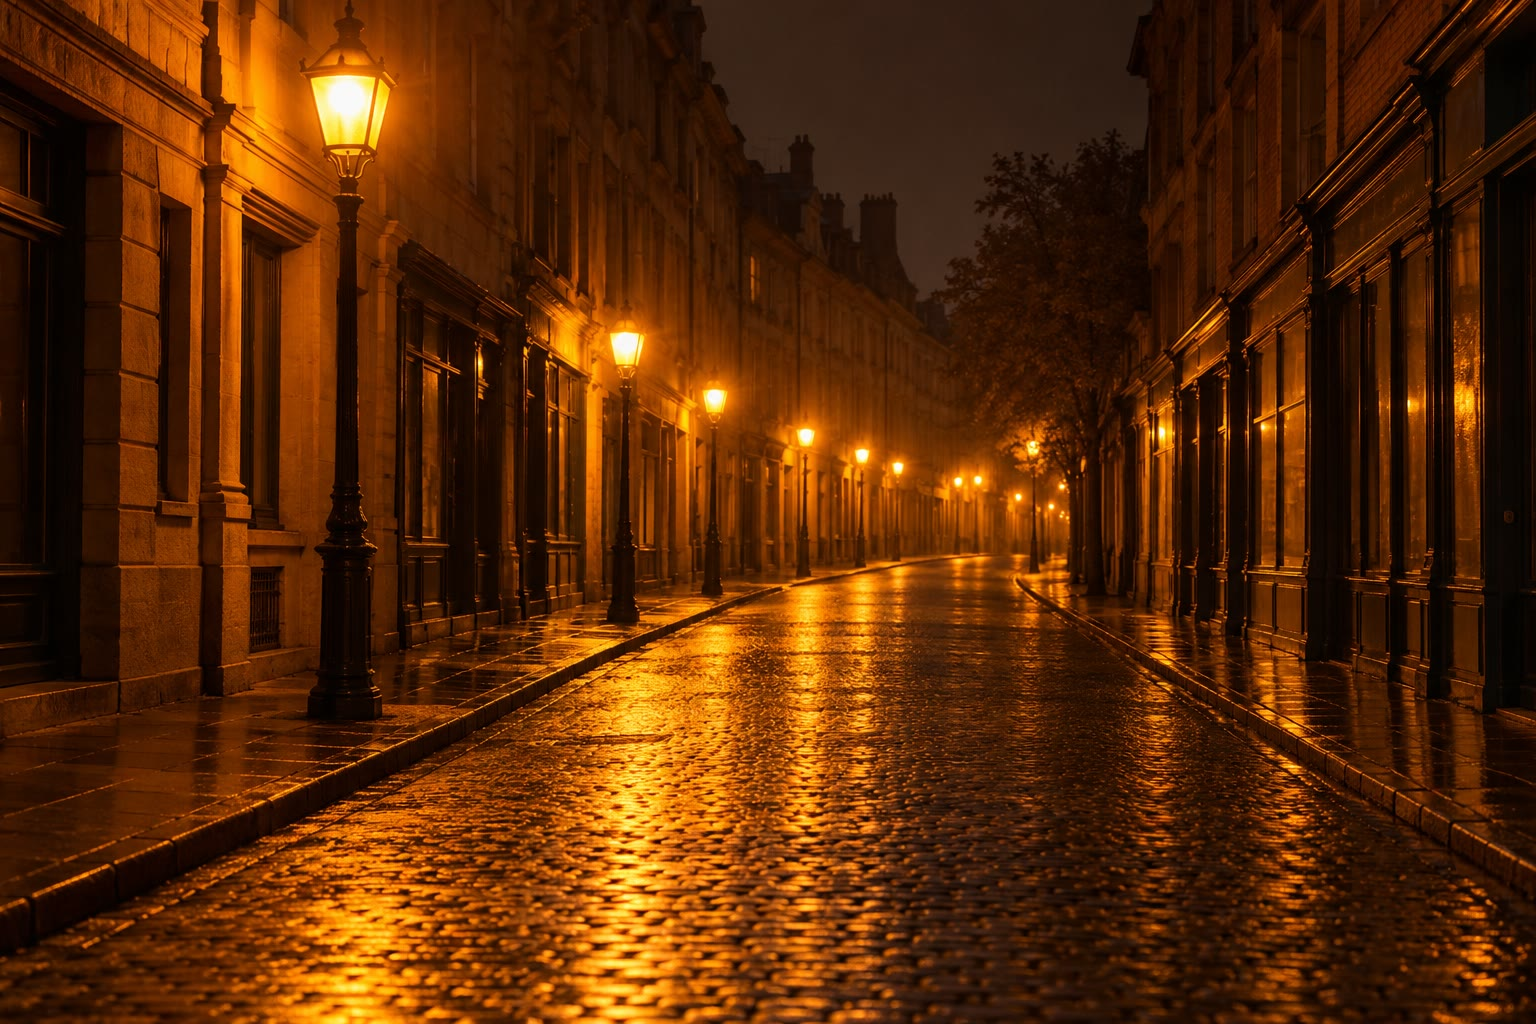
\includegraphics[width=0.62\linewidth]{images/book2/ai/b1-01-street-lamps.jpg}

{\small Low-pressure sodium street lamps. Their light is almost a single
orange-yellow line: like hydrogen, an excited sodium atom emits only
photons of a few precise energies.}
\end{omfigure}

\section{Quantised energies: the hydrogen spectrum}

\begin{definition}[Energy level, ground state, excited state]\label{def:b1:quantum-numbers:energy-level}
The energy of an electron bound in an atom can take only certain values,
the \emph{energy levels}\index{energy level} of the atom. The zero of
energy is taken when the electron is at rest infinitely far from the
nucleus (the atom is ionised), so every level of a bound electron is
negative. The lowest level is the \emph{ground state}\index{ground state};
every other level is an \emph{excited state}\index{excited state}.
\end{definition}

An atom passes from a level of energy $E_{\text{high}}$ to a lower level
$E_{\text{low}}$ by emitting one photon, and from the lower to the higher
level by absorbing one, of energy
\[
  h\nu = \frac{hc}{\lambda} = E_{\text{high}} - E_{\text{low}} .
\]
A spectrum of lines is therefore a picture of the differences between
the levels.

\begin{theorem}[Energy levels of the hydrogen atom]\label{thm:b1:quantum-numbers:levels}
The \omterm{def:b1:quantum-numbers:energy-level}{energy levels} of the hydrogen atom are
\[
  E_n = -\frac{E_R}{n^2}, \qquad n = 1, 2, 3, \dots,
  \qquad E_R = \qty{13.6}{eV},
\]
where $E_R$ is the Rydberg energy (corrected for the motion of the
nucleus). The \omterm{def:b1:quantum-numbers:energy-level}{ground state} is $E_1 = \qty{-13.6}{eV}$ and the ionisation
energy of the atom is $E_R$.
% ledger: const:RyhcEV, ie:H (13.598 eV; levels computed in
% figdata/bachelor-1/hydrogen-levels.py)
\end{theorem}
\admitted

\begin{remark}[Where the formula comes from]\label{rem:b1:quantum-numbers:schrodinger}
The formula follows from solving the Schrödinger equation of the electron
in the field of the proton; the solution, and the shapes of the
wavefunctions it gives, are derived in the Year 2 volume. Niels Bohr had
obtained the same levels in 1913 from a simpler model of circular orbits,
which is now abandoned.
\end{remark}

\begin{proposition}[The Rydberg formula]\label{prop:b1:quantum-numbers:rydberg}
The lines emitted by hydrogen have wavelengths given by
\[
  \frac{1}{\lambda} = R_H\left(\frac{1}{n_1^2} - \frac{1}{n_2^2}\right),
  \qquad n_2 > n_1 \ge 1, \qquad R_H = \frac{E_R}{hc},
\]
for the transition from level $n_2$ down to level $n_1$. The lines that
end on the same level $n_1$ form a \emph{series}: Lyman for $n_1 = 1$
(ultraviolet), Balmer for $n_1 = 2$ (visible), Paschen for $n_1 = 3$
(infrared).
\end{proposition}

\begin{proof}
The photon carries the energy lost by the atom:
$hc/\lambda = E_{n_2} - E_{n_1} = -E_R/n_2^2 + E_R/n_1^2
= E_R\,(1/n_1^2 - 1/n_2^2)$. Dividing by $hc$ gives the formula.
\end{proof}

\begin{example}[The red line of hydrogen]\label{ex:b1:quantum-numbers:halpha}
For the transition $3 \to 2$: $\Delta E = 13.6\,(1/4 - 1/9) =
\qty{1.89}{eV}$. With $hc = \qty{1240}{eV.nm}$ (from the values of $h$,
$c$ and $e$), $\lambda = 1240/1.89 = \qty{656}{nm}$: the red line.
The other Balmer lines, $4 \to 2$, $5 \to 2$, $6 \to 2$, fall at 486,
434 and \qty{410}{nm}; the next one, $7 \to 2$ at \qty{397}{nm}, is
already in the ultraviolet. The measured wavelengths, 656.3, 486.1, 434.0
and \qty{410.2}{nm}, agree to better than one part in two thousand; the
small remaining gap comes from measuring in air rather than in vacuum.
% ledger: asd:Halpha, asd:Hbeta, asd:Hgamma, asd:Hdelta (computed values
% in figdata/out/bachelor-1-hydrogen-levels-balmer.dat)
\end{example}

\begin{omfigure}
\begin{tikzpicture}
\begin{axis}[
  width=0.62\linewidth, height=7.2cm,
  xmin=0, xmax=10, ymin=-14.5, ymax=0.6,
  axis x line=none, axis y line=left,
  ylabel={energy (eV)}, ytick={-14,-12,-10,-8,-6,-4,-2,0},
  tick label style={font=\small}, label style={font=\small},
  clip=false]
\pgfplotsinvokeforeach{-13.598,-3.400,-1.511,-0.850,-0.544}{
  \draw[black!70, line width=0.7pt] (axis cs:0.3,#1) -- (axis cs:9.6,#1);}
\draw[black!40, dashed] (axis cs:0.3,0) -- (axis cs:9.6,0);
\node[font=\small, anchor=west] at (axis cs:9.7,-13.598) {$n = 1$};
\node[font=\small, anchor=west] at (axis cs:9.7,-3.400) {$n = 2$};
\node[font=\small, anchor=west] at (axis cs:9.7,-1.511) {$n = 3$};
\node[font=\small, anchor=south west] at (axis cs:9.7,0.05) {$n \to \infty$};
% Lyman
\draw[-{Stealth}, violet!70!black, thick] (axis cs:1.0,-3.400) -- (axis cs:1.0,-13.598);
\draw[-{Stealth}, violet!70!black, thick] (axis cs:1.6,-1.511) -- (axis cs:1.6,-13.598);
\draw[-{Stealth}, violet!70!black, thick] (axis cs:2.2,-0.850) -- (axis cs:2.2,-13.598);
\node[font=\small, violet!70!black, anchor=west] at (axis cs:2.4,-9) {Lyman};
% Balmer
\draw[-{Stealth}, red!80!black, thick] (axis cs:4.4,-1.511) -- (axis cs:4.4,-3.400);
\draw[-{Stealth}, teal!80!black, thick] (axis cs:5.0,-0.850) -- (axis cs:5.0,-3.400);
\draw[-{Stealth}, blue!80!black, thick] (axis cs:5.6,-0.544) -- (axis cs:5.6,-3.400);
\node[font=\small, anchor=north] at (axis cs:5.0,-3.6) {Balmer};
% Paschen
\draw[-{Stealth}, black!60, thick] (axis cs:7.8,-0.850) -- (axis cs:7.8,-1.511);
\draw[-{Stealth}, black!60, thick] (axis cs:8.4,-0.544) -- (axis cs:8.4,-1.511);
\node[font=\small, anchor=north] at (axis cs:8.1,-1.7) {Paschen};
\end{axis}
\end{tikzpicture}

{\small The \omterm{def:b1:quantum-numbers:energy-level}{energy levels} of hydrogen, $E_n = -\qty{13.6}{eV}/n^2$,
drawn to scale (computed from the Rydberg constant); the levels $n = 4,
5, \dots$ crowd below zero. Each arrow is one
emitted photon; arrows ending on the same level form a series.}
\end{omfigure}

\begin{omfigure}
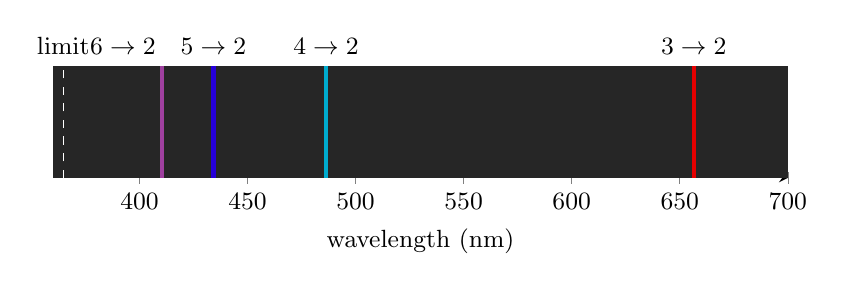
\begin{tikzpicture}
\begin{axis}[
  width=0.9\linewidth, height=3.0cm,
  xmin=360, xmax=700, ymin=0, ymax=1,
  axis x line=bottom, axis y line=none,
  xlabel={wavelength (nm)}, xtick={400,450,500,550,600,650,700},
  tick label style={font=\small}, label style={font=\small},
  clip=false]
\fill[black!85] (axis cs:360,0) rectangle (axis cs:700,1);
% line positions: figdata/out/bachelor-1-hydrogen-levels-balmer.dat
\draw[line width=1.6pt, red!90!black] (axis cs:656.5,0) -- (axis cs:656.5,1);
\draw[line width=1.6pt, cyan!80!green] (axis cs:486.3,0) -- (axis cs:486.3,1);
\draw[line width=1.6pt, blue!70!violet] (axis cs:434.2,0) -- (axis cs:434.2,1);
\draw[line width=1.6pt, violet!75] (axis cs:410.3,0) -- (axis cs:410.3,1);
\draw[white, dashed] (axis cs:364.7,0) -- (axis cs:364.7,1);
\node[font=\small, anchor=south] at (axis cs:364.7,1.02) {limit};
\node[font=\small, anchor=south] at (axis cs:656.5,1.02) {$3\to2$};
\node[font=\small, anchor=south] at (axis cs:486.3,1.02) {$4\to2$};
\node[font=\small, anchor=south] at (axis cs:434.2,1.02) {$5\to2$};
\node[font=\small, anchor=south east] at (axis cs:412,1.02) {$6\to2$};
\end{axis}
\end{tikzpicture}

{\small The Balmer lines computed from the Rydberg formula (vacuum
wavelengths), on the visible band. Further lines crowd towards the series
limit at \qty{364.7}{nm}, in the ultraviolet.}
\end{omfigure}

\begin{history}[Bohr's atom, 1913]
In 1913 Niels Bohr, a 28-year-old Danish physicist working in Manchester,
proposed that the electron of hydrogen could circle the nucleus only on
certain orbits, and that light was emitted when it jumped from one orbit
to a lower one. His model gave the Balmer lines exactly, and the value of
the Rydberg constant from $h$, $e$ and the mass of the electron. The
orbits did not survive the quantum mechanics of 1925--1926, but the
quantised levels did. Bohr received the Nobel Prize in Physics in 1922.
\end{history}

\begin{omfigure}
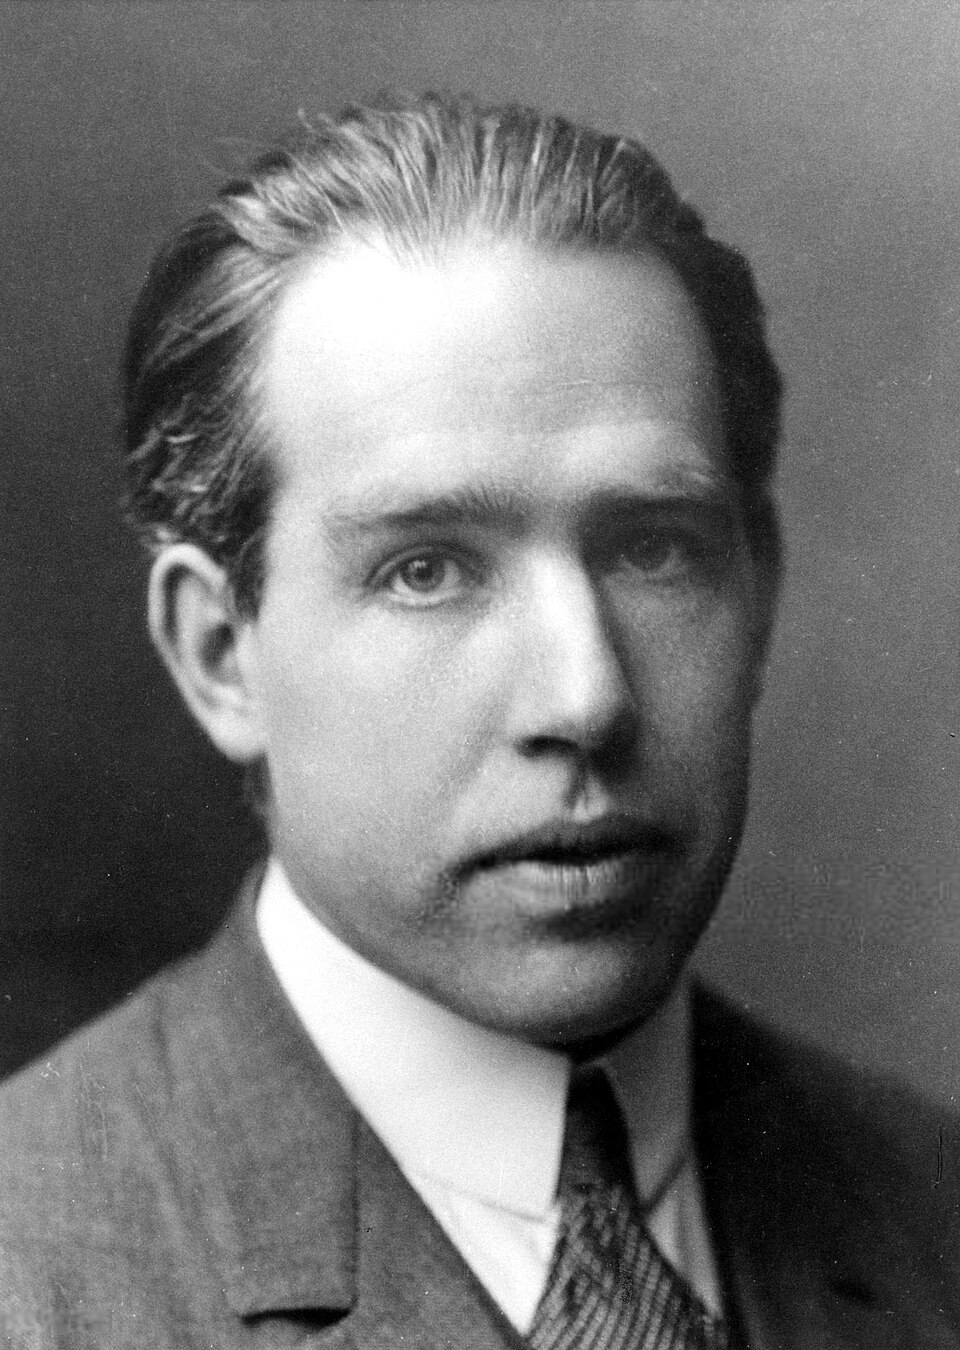
\includegraphics[width=0.26\linewidth]{images/book2/bohr.jpg}

{\small Niels Bohr (1885--1962), about 1922.}
\end{omfigure}

\section{Four quantum numbers}

In an atom with many electrons the energies are no longer given by a
single formula, but each electron is still described by a small set of
integers, its quantum numbers.

\begin{definition}[Quantum numbers]\label{def:b1:quantum-numbers:quantum-number}
The state of an electron in an atom is labelled by four numbers:
\begin{itemize}
  \item the \emph{principal quantum number}\index{principal quantum number}
        $n = 1, 2, 3, \dots$, which mainly fixes the energy and the size;
  \item the \emph{azimuthal quantum number}\index{azimuthal quantum number}
        (or secondary quantum number) $l = 0, 1, \dots, n-1$, which fixes
        the shape; $l = 0, 1, 2, 3$ are written s, p, d, f;
  \item the \emph{magnetic quantum number}\index{magnetic quantum number}
        $m_l = -l, -l+1, \dots, l$, which fixes the orientation ($2l + 1$
        values);
  \item the \emph{spin quantum number}\index{spin quantum number}
        $m_s = +\tfrac12$ or $-\tfrac12$, an intrinsic property of the
        electron, drawn as an arrow up or down.
\end{itemize}
\end{definition}

\begin{definition}[Atomic orbital, shell, subshell]\label{def:b1:quantum-numbers:orbital}
An \emph{atomic orbital}\index{atomic orbital} is the one-electron state
labelled by the three numbers $(n, l, m_l)$; it is drawn as one box,
\omorbs{}. The orbitals with the same $n$ form an \emph{electron
shell}\index{electron shell}; those with the same $n$ and $l$ form a
\emph{subshell}\index{subshell}, named by $n$ and the letter of $l$:
2p is the subshell $n = 2$, $l = 1$, made of three orbitals
($m_l = -1, 0, 1$).
\end{definition}

\begin{remark}[Shapes]\label{rem:b1:quantum-numbers:shapes}
An s orbital is spherical; a p orbital has two lobes along an axis, and
the three 2p orbitals point along $x$, $y$ and $z$. The mathematical
description of these shapes --- wavefunctions, their radial and angular
parts, their nodes --- belongs to the Year 2 volume. In this book an
orbital is a box that holds at most two electrons.
\end{remark}

\begin{proposition}[Capacity of a subshell and of a shell]\label{prop:b1:quantum-numbers:capacity}
A \omterm{def:b1:quantum-numbers:orbital}{subshell} of azimuthal number $l$ contains $2l + 1$ orbitals and can hold
$2(2l + 1)$ electrons: 2 in s, 6 in p, 10 in d, 14 in f. The shell $n$
contains $n^2$ orbitals and can hold $2n^2$ electrons.
\end{proposition}

\begin{proof}
For a given $l$, $m_l$ takes the $2l + 1$ values from $-l$ to $l$, and
each orbital holds two electrons of opposite spins (\cref{prop:b1:quantum-numbers:pauli}
below). For a given $n$, $l$ runs from $0$ to $n - 1$, so the number of
orbitals is
\[
  \sum_{l=0}^{n-1} (2l+1) = 2\,\frac{(n-1)n}{2} + n = n^2 ,
\]
and the number of electrons is $2n^2$: 2, 8, 18, 32 for $n = 1$ to 4.
\end{proof}

\begin{example}[The third shell]\label{ex:b1:quantum-numbers:third}
For $n = 3$: $l = 0$ (3s, one orbital), $l = 1$ (3p, three orbitals),
$l = 2$ (3d, five orbitals, $m_l = -2, \dots, 2$): nine orbitals and up
to 18 electrons. An electron in 3d has, for instance, the quantum
numbers $(3, 2, -1, +\tfrac12)$.
\end{example}

\section{Building configurations}

\begin{definition}[Electron configuration]\label{def:b1:quantum-numbers:configuration}
The \emph{electron configuration}\index{electron configuration} of an
atom or ion is the list of its occupied \omterm{def:b1:quantum-numbers:orbital}{subshells} with the number of
electrons in each, written as an exponent: $1\text{s}^2 2\text{s}^2
2\text{p}^4$ for oxygen. The electrons of the highest $n$, together with
those of an incompletely filled d or f \omterm{def:b1:quantum-numbers:orbital}{subshell}, are the \emph{valence
electrons}\index{valence electrons}; the others are the \emph{core
electrons}\index{core electrons}. A configuration is abbreviated by
writing the configuration of the preceding noble gas in brackets:
oxygen is $[\ce{He}]\,2\text{s}^2 2\text{p}^4$.
\end{definition}

Three rules give the ground-state configuration.

\begin{proposition}[Pauli exclusion principle]\label{prop:b1:quantum-numbers:pauli}
Two electrons of the same atom never have the same four quantum numbers.
Hence one orbital holds at most two electrons, and then with opposite
spins: \omorbs{ud}.
\end{proposition}
\admitted

\begin{proposition}[Klechkowski rule]\label{prop:b1:quantum-numbers:klechkowski}
In the \omterm{def:b1:quantum-numbers:energy-level}{ground state} of a neutral atom, \omterm{def:b1:quantum-numbers:orbital}{subshells} are filled in the order
of increasing $n + l$, and for equal $n + l$ in the order of increasing
$n$:
\[
  1\text{s},\ 2\text{s},\ 2\text{p},\ 3\text{s},\ 3\text{p},\ 4\text{s},\
  3\text{d},\ 4\text{p},\ 5\text{s},\ 4\text{d},\ 5\text{p},\ 6\text{s},\
  4\text{f},\ 5\text{d},\ 6\text{p},\ 7\text{s},\ 5\text{f},\ 6\text{d},\
  7\text{p}.
\]
\end{proposition}
\admitted

\begin{remark}[An empirical rule]\label{rem:b1:quantum-numbers:klech-empirical}
The Klechkowski rule (also called the Madelung rule) is a summary of
observed configurations, not a law: it describes the order in which the
\omterm{def:b1:quantum-numbers:orbital}{subshells} fill as the nuclear charge increases. In an atom with many
electrons, the electrons repel one another, so the energy of a \omterm{def:b1:quantum-numbers:orbital}{subshell}
depends on $l$ as well as $n$: a 4s electron, which spends part of its
time close to the nucleus, ends up below 3d in potassium and calcium.
\end{remark}

\begin{omfigure}
\begin{tikzpicture}[font=\small, x=1.25cm, y=0.72cm]
  \foreach \n in {1,...,7} {
    \foreach \l/\s in {0/s,1/p,2/d,3/f} {
      \pgfmathtruncatemacro\ok{(\l<\n) && (\n+\l<=8)}
      \ifnum\ok=1
        \node[draw=black!50, rounded corners=2pt, minimum width=0.85cm,
          minimum height=0.5cm, fill=white] (s\n\l) at (\l,-\n) {\n\s};
      \fi
    }
  }
  \begin{scope}[on background layer]
  \foreach \la/\na/\lb/\nb in {0/1/0/1, 0/2/0/2, 1/2/0/3, 1/3/0/4, 2/3/0/5,
      2/4/0/6, 3/4/0/7, 3/5/1/7} {
    \draw[-{Stealth}, omDef, thick, opacity=0.8]
      ($(\la,-\na)+(0.5,0.42)$) -- ($(\lb,-\nb)+(-0.5,-0.42)$);
  }
  \end{scope}
  \node[anchor=west, align=left, font=\small] at (4.0,-2.5) {follow each arrow,\\then the next one\\to its right};
\end{tikzpicture}

{\small The Klechkowski diagram. The \omterm{def:b1:quantum-numbers:orbital}{subshells} of the same $n + l$ lie on
one diagonal; following the diagonals in order gives the filling order
1s, 2s, 2p, 3s, 3p, 4s, 3d, 4p, 5s, \dots}
\end{omfigure}

\begin{proposition}[Hund's rule]\label{prop:b1:quantum-numbers:hund}
When the electrons of a \omterm{def:b1:quantum-numbers:orbital}{subshell} can be placed in several orbitals of
the same energy, the \omterm{def:b1:quantum-numbers:energy-level}{ground state} has the largest number of
\emph{parallel} spins: the electrons occupy separate orbitals, spins
up, before any orbital is doubly filled.
\end{proposition}
\admitted

\begin{definition}[Unpaired electron]\label{def:b1:quantum-numbers:unpaired}
An \emph{unpaired electron}\index{unpaired electron} is an electron
alone in its orbital. A species with unpaired electrons is attracted by a
magnet (it is paramagnetic, a property studied in physics).
\end{definition}

\begin{method}[Writing a ground-state configuration]\label{met:b1:quantum-numbers:configuration}
To write the configuration of an atom of atomic number $Z$:
\begin{enumerate}
  \item place $Z$ electrons in the \omterm{def:b1:quantum-numbers:orbital}{subshells} in the Klechkowski order,
        filling each \omterm{def:b1:quantum-numbers:orbital}{subshell} (2, 6, 10, 14) before the next;
  \item write the result in the order of increasing $n$ (grouping 3d
        with $n = 3$), and abbreviate with the core of the preceding
        noble gas;
  \item for the last, incompletely filled \omterm{def:b1:quantum-numbers:orbital}{subshell}, draw the boxes and
        apply Hund's rule to count the \omterm{def:b1:quantum-numbers:unpaired}{unpaired electrons}.
\end{enumerate}
\end{method}

\begin{example}[Carbon, nitrogen, oxygen, iron]\label{ex:b1:quantum-numbers:examples}
The method gives, for four atoms:
\begin{center}
\begin{tabular}{lllc}
\hline
atom & configuration & last \omterm{def:b1:quantum-numbers:orbital}{subshell} & unpaired \\
\hline
\ce{C} ($Z = 6$) & $[\ce{He}]\,2\text{s}^2 2\text{p}^2$ & 2p: \omorbs{u,u,} & 2 \\
\ce{N} ($Z = 7$) & $[\ce{He}]\,2\text{s}^2 2\text{p}^3$ & 2p: \omorbs{u,u,u} & 3 \\
\ce{O} ($Z = 8$) & $[\ce{He}]\,2\text{s}^2 2\text{p}^4$ & 2p: \omorbs{ud,u,u} & 2 \\
\ce{Fe} ($Z = 26$) & $[\ce{Ar}]\,3\text{d}^6 4\text{s}^2$ & 3d: \omorbs{ud,u,u,u,u} & 4 \\
\hline
\end{tabular}
\end{center}
For iron the Klechkowski order fills 4s ($Z = 19, 20$) before 3d
($Z = 21$ to 30); the configuration is written with 3d first.
% ledger: gs:Fe
\end{example}

\begin{omfigure}
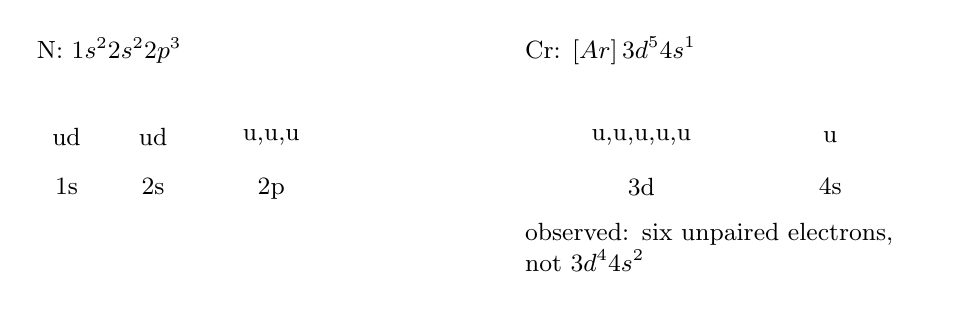
\begin{tikzpicture}[font=\small]
  \begin{scope}
    \node[anchor=west] at (0,2.4) {\ce{N}: $1\text{s}^2 2\text{s}^2 2\text{p}^3$};
    \node at (0.5,1.3) {\omorbs{ud}}; \node[below] at (0.5,0.9) {1s};
    \node at (1.6,1.3) {\omorbs{ud}}; \node[below] at (1.6,0.9) {2s};
    \node at (3.1,1.3) {\omorbs{u,u,u}}; \node[below] at (3.1,0.9) {2p};
  \end{scope}
  \begin{scope}[xshift=6.2cm]
    \node[anchor=west] at (0,2.4) {\ce{Cr}: $[\ce{Ar}]\,3\text{d}^5 4\text{s}^1$};
    \node at (1.6,1.3) {\omorbs{u,u,u,u,u}}; \node[below] at (1.6,0.9) {3d};
    \node at (4.0,1.3) {\omorbs{u}}; \node[below] at (4.0,0.9) {4s};
    \node[anchor=west, text width=5.0cm] at (0,-0.1) {observed: six unpaired electrons, not $3\text{d}^4 4\text{s}^2$};
  \end{scope}
\end{tikzpicture}

{\small Quantum boxes. Each box is one orbital; an arrow is one electron
and its spin. Nitrogen follows Hund's rule; chromium is one of the
exceptions of \cref{prop:b1:quantum-numbers:exceptions}.}
\end{omfigure}

\section{Ions, exceptions and the shape of the table}

\begin{proposition}[Configurations of ions]\label{prop:b1:quantum-numbers:ions}
A monatomic anion has the configuration of the atom with the extra
electrons added in the next places of the Klechkowski order; a cation of a
main-group element loses the electrons of highest $n$. A cation of a
transition metal loses its $n$s electrons \emph{before} its
$(n-1)$d electrons: \ce{Fe^{2+}} is $[\ce{Ar}]\,3\text{d}^6$ and
\ce{Fe^{3+}} is $[\ce{Ar}]\,3\text{d}^5$, not $[\ce{Ar}]\,3\text{d}^4
4\text{s}^2$.
% ledger: gs:Fe2+, gs:Fe3+
\end{proposition}
\admitted

\begin{remark}[Filling order is not removal order]\label{rem:b1:quantum-numbers:order}
4s fills before 3d in potassium and calcium, yet it is emptied first in
the transition-metal ions. There is no contradiction: the order of the
\omterm{def:b1:quantum-numbers:orbital}{subshell} energies changes with the nuclear charge and the number of
electrons, and in a transition-metal atom or ion the 3d \omterm{def:b1:quantum-numbers:orbital}{subshell} lies
below 4s. The Klechkowski rule describes neutral atoms only.
\end{remark}

\begin{proposition}[Two exceptions in the first transition series]\label{prop:b1:quantum-numbers:exceptions}
The observed ground-state configurations of chromium and copper are
\[
  \ce{Cr}: [\ce{Ar}]\,3\text{d}^5 4\text{s}^1, \qquad
  \ce{Cu}: [\ce{Ar}]\,3\text{d}^{10} 4\text{s}^1 ,
\]
instead of $3\text{d}^4 4\text{s}^2$ and $3\text{d}^9 4\text{s}^2$
predicted by the Klechkowski rule: a half-filled or filled d \omterm{def:b1:quantum-numbers:orbital}{subshell} is
especially stable, and the 4s and 3d levels are close.
% ledger: gs:Cr, gs:Cu
\end{proposition}

\begin{example}[Copper and its ions]\label{ex:b1:quantum-numbers:copper}
\ce{Cu} is $[\ce{Ar}]\,3\text{d}^{10} 4\text{s}^1$; \ce{Cu+} is
$[\ce{Ar}]\,3\text{d}^{10}$, with no \omterm{def:b1:quantum-numbers:unpaired}{unpaired electron}; \ce{Cu^{2+}} is
$[\ce{Ar}]\,3\text{d}^9$, with one. \ce{Zn^{2+}}, $[\ce{Ar}]\,3\text{d}^{10}$,
has none.
% ledger: gs:Cu+, gs:Cu2+, gs:Zn2+
\end{example}

\begin{proposition}[Configurations and the periodic table]\label{prop:b1:quantum-numbers:table}
Period $n$ of the periodic table begins with the filling of $n$s and ends
with the filling of $n$p. The \omterm{def:b1:quantum-numbers:orbital}{subshells} filled in between are, by the
Klechkowski rule, $(n-2)$f and $(n-1)$d. Hence the periods hold
$2, 8, 8, 18, 18, 32, 32$ elements, and the noble gases have $Z = 2, 10,
18, 36, 54, 86, 118$.
\end{proposition}

\begin{proof}
Periods 1 to 3 contain only $n$s (and $n$p for $n \ge 2$): $2$, then
$2 + 6 = 8$ twice. In periods 4 and 5, $(n-1)$d is added: $2 + 10 + 6 =
18$. In periods 6 and 7, $(n-2)$f as well: $2 + 14 + 10 + 6 = 32$. The
noble gases close each period: $2$, $2 + 8 = 10$, $18$, $18 + 18 = 36$,
$54$, $54 + 32 = 86$, $118$.
\end{proof}

\begin{omfigure}
\omperiodictable[colour=blocks, legend]

{\small The periodic table coloured by the last \omterm{def:b1:quantum-numbers:orbital}{subshell} being filled:
the s, p, d and f blocks. The width of each block is the capacity of its
\omterm{def:b1:quantum-numbers:orbital}{subshell}, 2, 6, 10 and 14.}
\end{omfigure}

\section{Exercises}

\begin{exercise}[$\star$]\label{exo:b1:quantum-numbers:1}
Which of these sets $(n, l, m_l, m_s)$ can describe an electron in an
atom? Explain each refusal.
(a) $(2, 2, 0, +\tfrac12)$; (b) $(3, 1, -1, -\tfrac12)$;
(c) $(1, 0, 0, 0)$; (d) $(4, 3, -3, +\tfrac12)$; (e) $(3, 0, 1, -\tfrac12)$.
\end{exercise}

\begin{exercise}[$\star$]\label{exo:b1:quantum-numbers:2}
How many orbitals, and at most how many electrons, are there in the
\omterm{def:b1:quantum-numbers:orbital}{subshells} 3d, 4f and 5p, and in the shell $n = 2$?
\end{exercise}

\begin{exercise}[$\star$]\label{exo:b1:quantum-numbers:3}
Write the ground-state configurations of \ce{O}, \ce{P}, \ce{K}, \ce{Ca}
and \ce{Br} ($Z = 8, 15, 19, 20, 35$), in full and abbreviated, and give
the number of \omterm{def:b1:quantum-numbers:configuration}{valence electrons} of each.
\end{exercise}

\begin{exercise}[$\star$]\label{exo:b1:quantum-numbers:4}
Draw the quantum boxes of the valence \omterm{def:b1:quantum-numbers:orbital}{subshells} of nitrogen, sulfur and
chlorine, and count their \omterm{def:b1:quantum-numbers:unpaired}{unpaired electrons}.
\end{exercise}

\begin{exercise}[$\star\star$]\label{exo:b1:quantum-numbers:5}
Give the configurations of \ce{Na+}, \ce{Mg^{2+}}, \ce{Al^{3+}}, \ce{F-},
\ce{O^{2-}}, \ce{Cl-}, \ce{S^{2-}} and \ce{Ca^{2+}}. Which noble gas is
each isoelectronic with?
\end{exercise}

\begin{exercise}[$\star\star$]\label{exo:b1:quantum-numbers:6}
Write the configurations of \ce{Ti^{2+}}, \ce{Mn^{2+}}, \ce{Co^{2+}},
\ce{Ni^{2+}} and \ce{Zn^{2+}} ($Z = 22, 25, 27, 28, 30$) and give the
number of \omterm{def:b1:quantum-numbers:unpaired}{unpaired electrons} of each.
\end{exercise}

\begin{exercise}[$\star\star$]\label{exo:b1:quantum-numbers:7}
Compute the energy and the wavelength of the photon emitted in the
transition $4 \to 3$ of hydrogen. In which part of the spectrum is it?
Take $E_R = \qty{13.6}{eV}$ and $hc = \qty{1240}{eV.nm}$.
\end{exercise}

\begin{exercise}[$\star\star$]\label{exo:b1:quantum-numbers:8}
Identify the elements whose ground-state configurations end in
(a) $3\text{s}^2 3\text{p}^4$; (b) $4\text{s}^2 3\text{d}^{10} 4\text{p}^5$;
(c) $5\text{s}^1$; (d) $4\text{s}^2 3\text{d}^3$. Give the four quantum
numbers of one electron of the last \omterm{def:b1:quantum-numbers:orbital}{subshell} of (a).
\end{exercise}

\begin{exercise}[$\star\star$]\label{exo:b1:quantum-numbers:9}
Using the Klechkowski rule, explain why the nineteenth electron of
potassium goes into 4s and not into 3d, and why period 3 holds 8
elements and not 18.
\end{exercise}

\begin{exercise}[$\star\star\star$]\label{exo:b1:quantum-numbers:10}
An ion with a single electron and a nucleus of charge $Ze$ has levels
$E_n = -Z^2 E_R/n^2$ (admitted). For \ce{He+} ($Z = 2$), compute the
ionisation energy and the wavelength of the transition $2 \to 1$.
Compare with hydrogen.
\end{exercise}

\begin{exercise}[$\star\star\star$]\label{exo:b1:quantum-numbers:11}
Say whether each configuration is a \omterm{def:b1:quantum-numbers:energy-level}{ground state}, an \omterm{def:b1:quantum-numbers:energy-level}{excited state} or
impossible, and why: (a) $1\text{s}^2 2\text{s}^1 2\text{p}^1$;
(b) $1\text{s}^2 2\text{s}^2 2\text{p}^7$; (c) $1\text{s}^2 2\text{p}^2$;
(d) $[\ce{Ne}]\,3\text{s}^2 3\text{p}^3$; (e) $1\text{s}^3$.
\end{exercise}

\begin{exercise}[$\star\star\star$]\label{exo:b1:quantum-numbers:12}
Iron(III) salts are attracted by a magnet more strongly than iron(II)
salts, and zinc salts not at all. Rank \ce{Fe^{2+}}, \ce{Fe^{3+}},
\ce{Mn^{2+}}, \ce{Cu^{2+}} and \ce{Zn^{2+}} by number of \omterm{def:b1:quantum-numbers:unpaired}{unpaired
electrons}, and explain the observation, assuming the attraction grows
with that number.
\end{exercise}

\section{Problem: Lines of a Lamp, and a World with Three Spins}

\begin{problem}[{Weekend problem --- from the four lines of a hydrogen
lamp to the length of the periods, and what the table would look like
if an electron had three spin states}]
\label{pb:b1:quantum-numbers:1}
Take $E_R = \qty{13.6}{eV}$ and $hc = \qty{1240}{eV.nm}$ throughout.
The visible band runs from about 400 to \qty{700}{nm}.

\medskip
\noindent\textbf{Part I --- The hydrogen lamp.}
\begin{enumerate}
  \item Compute the energies $E_1$ to $E_4$ of the hydrogen atom.
  \item Compute the energy and the wavelength of the photon emitted in
        the transition $3 \to 2$. What is its colour?
  \item Compute the wavelengths of the transitions $4 \to 2$, $5 \to 2$
        and $6 \to 2$.
  \item Why does a hydrogen lamp show exactly four visible lines?
        Compute the wavelength of $7 \to 2$ to support the answer.
  \item Compute the series limit of the Balmer series.
  \item Compute the wavelength of the first Lyman line, $2 \to 1$. Why can
        it not be seen?
  \item What is the longest wavelength of a photon able to ionise a
        hydrogen atom in its \omterm{def:b1:quantum-numbers:energy-level}{ground state}?
\end{enumerate}

\medskip
\noindent\textbf{Part II --- Counting states.}
\begin{enumerate}[resume]
  \item List the values of $l$ and $m_l$ for $n = 3$; how many orbitals
        does the shell hold?
  \item Show that the shell $n$ holds $2n^2$ electrons; apply to $n = 4$.
  \item Write the Klechkowski order up to 7p.
  \item Deduce the lengths of the seven periods.
  \item Explain why the 3d \omterm{def:b1:quantum-numbers:orbital}{subshell} does not appear in period 3.
  \item Deduce the atomic numbers of the noble gases.
\end{enumerate}

\medskip
\noindent\textbf{Part III --- The transition metals.}
\begin{enumerate}[resume]
  \item Write the configuration of iron ($Z = 26$) and draw its 3d
        boxes. How many \omterm{def:b1:quantum-numbers:unpaired}{unpaired electrons}?
  \item Same questions for \ce{Fe^{2+}} and \ce{Fe^{3+}}. Which of the two
        has a half-filled \omterm{def:b1:quantum-numbers:orbital}{subshell}?
  \item The observed configuration of chromium is $[\ce{Ar}]\,3\text{d}^5
        4\text{s}^1$. Compare with the prediction, and count the \omterm{def:b1:quantum-numbers:unpaired}{unpaired
        electrons} in each.
  \item Give the configurations of \ce{Cu}, \ce{Cu+} and \ce{Cu^{2+}}.
  \item Which of \ce{Cu+} and \ce{Cu^{2+}} has \omterm{def:b1:quantum-numbers:unpaired}{unpaired electrons}?
  \item Among \ce{Sc^{3+}}, \ce{Ti^{3+}}, \ce{Mn^{2+}} ($Z = 21, 22, 25$),
        which has the most \omterm{def:b1:quantum-numbers:unpaired}{unpaired electrons}?
\end{enumerate}

\medskip
\noindent\textbf{Part IV --- A world with three spins.}
Imagine a universe where $n$, $l$ and $m_l$ obey the same rules as in
ours, the Klechkowski order is unchanged, the exclusion principle holds,
but the spin number $m_s$ can take three values.
\begin{enumerate}[resume]
  \item How many electrons can one orbital hold? A \omterm{def:b1:quantum-numbers:orbital}{subshell} of number
        $l$? A shell $n$?
  \item Give the capacities of 1s, 2s, 2p, 3s and 3p.
  \item A noble gas closes a period with a filled p \omterm{def:b1:quantum-numbers:orbital}{subshell} (or 1s for
        the first). What is the atomic number of the first noble gas?
  \item Which atomic number would behave like an alkali metal, with a
        single electron beyond the first noble gas?
  \item How many elements would the second period hold?
  \item Compute the atomic number of the second noble gas of this world.
\end{enumerate}
\end{problem}
